\section{Lepton Universality Tests}
\subsection{The Electroweak Sector}
\frame{\tableofcontents[currentsection]}
    \begin{frame}{Partial Width of the Z-Boson}
        \begin{columns}
            \begin{column}{0.5\textwidth}
                \begin{itemize}
                    \item compare partial widths \rightarrow ratios
                    \begin{itemize}
                        \item no favoured flavour
                        \item [\rightarrow] expect ratios near 1
                    \end{itemize} 
                    \item measurements \footnotemark{} \footnotemark{} :
                    \begin{itemize}
                        \item [] <2, 3, 4 >$\frac{\Gamma_{Z \rightarrow \mu^+ \mu^-}}{\Gamma_{Z \rightarrow e^+ e^-}} = 1.0009 \pm 0.0028$
                        \item  []
                        \item [] <3, 4 > $\frac{\Gamma_{Z \rightarrow \tau^+ \tau^-}}{\Gamma_{Z \rightarrow e^+ e^-}} = 1.0019 \pm 0.0032$
                        \item []
                        \item [] <4>$\frac{\Gamma_{Z \rightarrow \mu^+ \mu^-}}{\Gamma_{Z \rightarrow e^+ e^-}} = 0.9974 \pm 0.0050$
                        %
                    \end{itemize}
                \end{itemize}
            \end{column}
            \begin{column}{0.5\textwidth}
                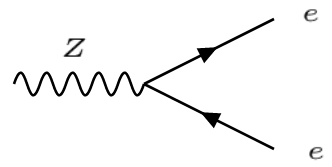
\includegraphics[width = 0.42\textwidth]{content/images/Zdecay_ee.png} \\
                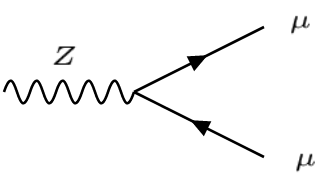
\includegraphics[width = 0.42\textwidth]{content/images/Zdecay_mumu.png} \\
                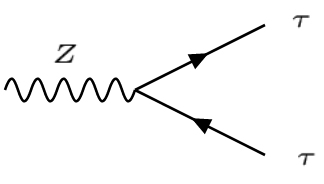
\includegraphics[width = 0.42\textwidth]{content/images/Zdecay_tautau.png}
            \end{column}
        \end{columns}
        \stepcounter{footnote} \footnotetext{arXiv:hep-ex/0509008}
        \stepcounter{footnote} \footnotetext{arXiv:1612.03016}
    \end{frame}
    \begin{frame}{Partials Widths of the $W^{\pm}$-Boson}
        \begin{columns}
            \begin{column}{0.5\textwidth}
              \begin{itemize}
                \item compare partial widths \rightarrow ratios
                \begin{itemize}
                    \item no favoured flavour
                    \item [\rightarrow] expect ratios near 1
                \end{itemize} 
                \item measurements \footnotemark{} :
                \begin{itemize}
                    \item [] < 2, 3, 4, 5> $\frac{\Gamma_{W \rightarrow \tau^- \bar{\nu}_\tau}}{\Gamma_{W \rightarrow e^- \bar{\nu}_e }} = 1.063 \pm 0.027$
                    \item  []
                    \item [] < 3, 4, 5> $\frac{\Gamma_{W \rightarrow \tau^- \bar{\nu}_\tau}}{\Gamma_{W \rightarrow \mu^- \bar{\nu}_\mu }} = 1.070 \pm 0.026$
                    \item []
                    \item [] <4, 5>$\frac{2\Gamma_{W \rightarrow \tau^- \bar{\nu}_\tau}}{\Gamma_{W \rightarrow \mu^- \bar{\nu}_\mu } + \Gamma_{W \rightarrow e^- \bar{\nu}_e }} = 1.066 \pm 0.025$
                \end{itemize}
                \item <5> $\approx 2.3 \sigma $ deviation!
            \end{itemize}
            \end{column}
            \begin{column}{0.5\textwidth}
                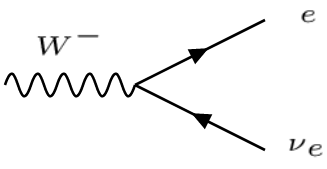
\includegraphics[width = 0.42\textwidth]{content/images/Wdecay_e.png} \\
                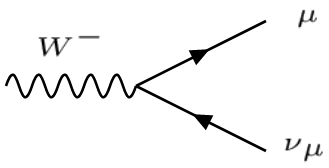
\includegraphics[width = 0.42\textwidth]{content/images/Wdecay_mu.png} \\
                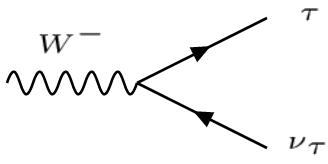
\includegraphics[width = 0.42\textwidth]{content/images/Wdecay_tau.png}
            \end{column}
        \end{columns}
        \stepcounter{footnote}\footnotetext{arXiv:1302.3415}
    \end{frame}

    \begin{frame}{Difficulty: tau reconstruction}
        \begin{columns}
            \begin{column}{0.45\textwidth}
                \begin{itemize}
                    \item channels
                    \begin{itemize}
                        \item $ \tau_l$
                        \item $ \tau_{\text{had}}$
                    \end{itemize}
                    \visible<2, 3, 4>{ \item $\tau_{\text{had}}$ means a hadronically decaying tau-leptons
                    \begin{itemize}
                        \item no visible jets
                        \item decay products form pions 
                    \end{itemize}}
                    \visible<3, 4>{
                    \item $\tau_{\text{lep}}$ means leptonically decaying tau-leptons
                    \begin{itemize}
                        \item two neutrinos \textrightarrow difficult to reconstruct
                        \item only leptons (e, $\mu$) visible
                    \end{itemize}}
                    \item <4> may be cause of deviation
                \end{itemize}
            \end{column}
    
            \begin{column}{0.55\textwidth}{Branching Ratios of the $W^{\pm}$-Boson}
                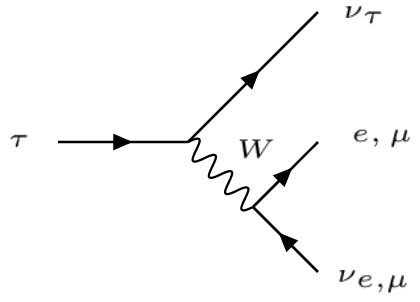
\includegraphics[scale=0.3]{content/feynman/png/tau_lep.png}
                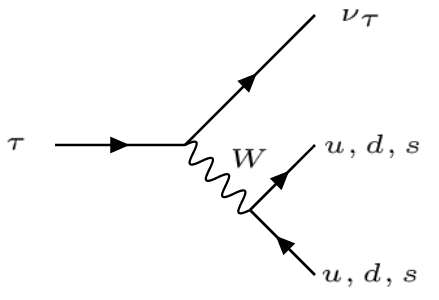
\includegraphics[scale=0.3]{content/feynman/png/tau_had.png}
            \end{column}
    
        \end{columns}
    \end{frame}

    \begin{frame}
        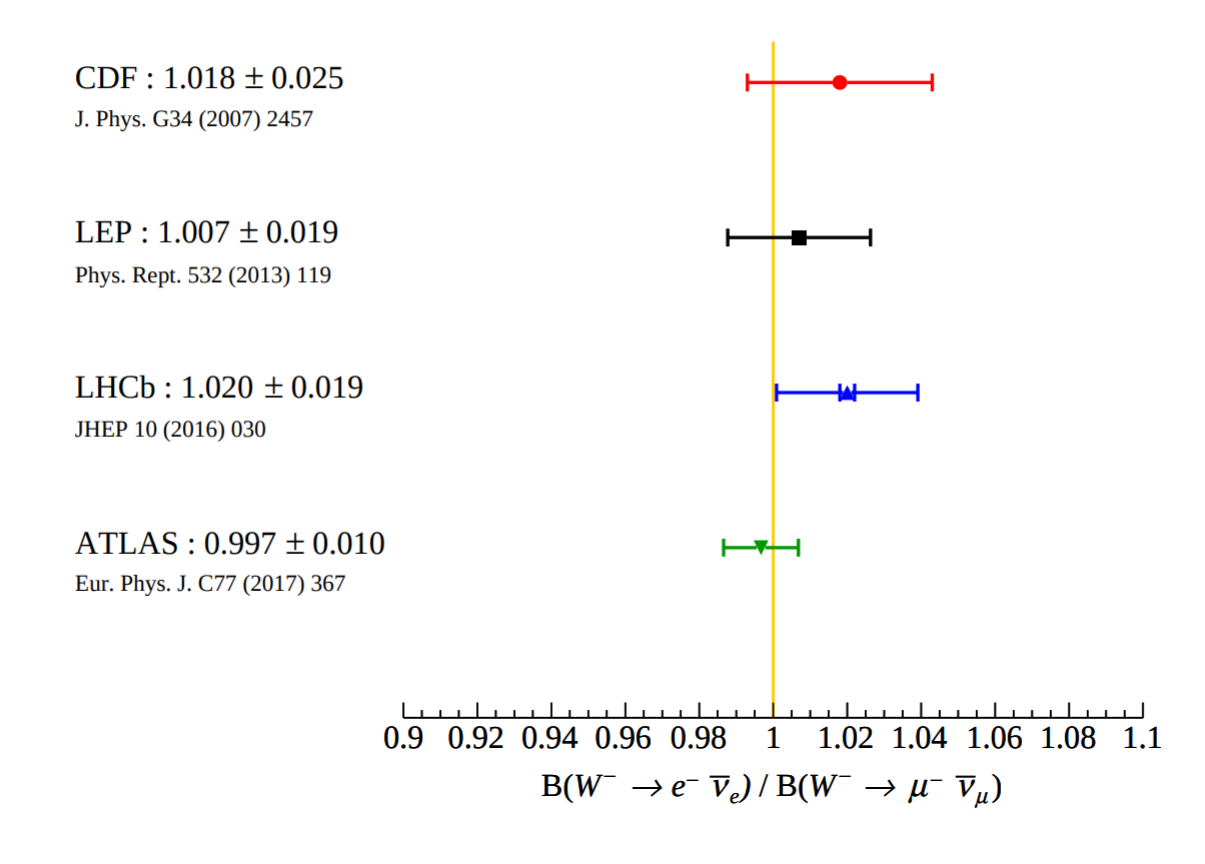
\includegraphics[width=0.75\textwidth]{content/images/BR_W.png}
    \end{frame}

\subsection{Pseudoscalar Mesons}
\frame{\tableofcontents[currentsection]}
\begin{frame}{Pseudoscalar Mesons}
    \begin{columns}[T]
        \begin{column}{0.7\textwidth}
            \begin{itemize}
                \item study decay of $\pi^-$
                \begin{itemize}
                    \item composed of $d, \bar{u} $
                    \item Spin 0
                    \visible<2, 3, 4, 5>{\item [\rightarrow] consider helicity}
                \end{itemize}
                \item 
                 \begin{align*}
                    \left(\frac{\Gamma_{\pi^- \rightarrow e^- \bar{\nu}_e}}{\Gamma_{\pi^- \rightarrow \mu^- \bar{\nu}_\mu}} \right)^{SM} \only<1, 2>{\neq 1 } \visible<3, 4, 5>{ &= \left(\frac{M_e}{M_\mu} \right)^2 \frac{M^2_\pi - M^2_e}{M^2_\pi - M^2_\mu}(1 +\delta_\text{QED} )  \\
                    \visible<4, 5>{ &= (1.2352 \pm 0.0001)\cdot 10^{-4}} }
                \end{align*}
               \visible<5>{ \item measured :
                \begin{itemize}
                    \item $\frac{\Gamma_{\pi^- \rightarrow e^- \bar{\nu}_e}}{\Gamma_{\pi^- \rightarrow \mu^- \bar{\nu}_\mu}} = (1.230 \pm 0.004) \cdot 10^{-4} $
                \end{itemize}}
            \end{itemize}
        \end{column}
        %------------%
        \begin{column}{0.4\textwidth}
            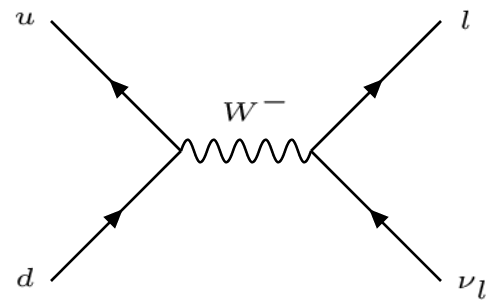
\includegraphics[width = 0.7\textwidth]{content/images/pi_l.png} \\
            \visible<2, 3, 4, 5>{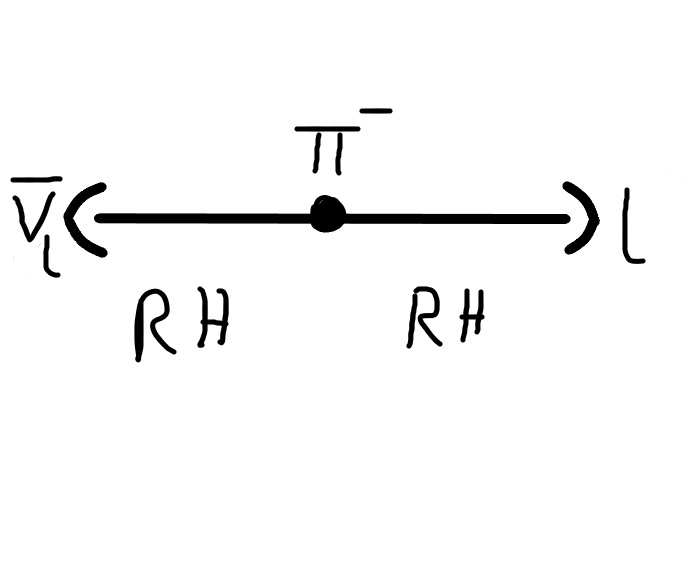
\includegraphics[width = 0.8\textwidth]{content/images/pi_hel.png}} 
            %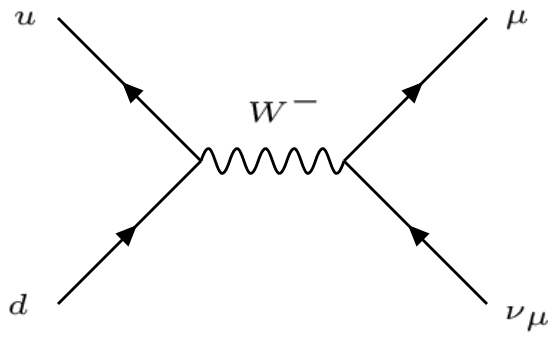
\includegraphics[width = 0.7\textwidth]{content/images/pi_mu.png} 
        \end{column}
    \end{columns}
    
\end{frame}

\subsection{Meson Mixing}
\begin{frame}{$R_{K}$ and $R_{K^*}$}
    \begin{columns}
        \begin{column}{0.5\textwidth}
            \begin{itemize}
                \item anomalies in $\bar{B}^{0} \rightarrow \bar{H} l \bar{l}$ 
                \begin{itemize}
                    \item $H = K, K^*$
                \end{itemize} 
                \item <2, 3, 4> $R_{K} = \frac{ \displaystyle \int_{q^2_{min}}^{q^2_{max}} \frac{\symup{d}\mathcal{B} [ B \rightarrow H \mu^+ \mu^- ] } {\symup{d}q^2} } {\displaystyle \int_{q^2_{min}}^{q^2_{max}} \frac{\symup{d}\mathcal{B} [ B \rightarrow H e^+ e^- ] } {\symup{d}q^2}} \stackrel{!}{=} 1$ 
                \item <3, 4> LHCb \footnotemark:
                \begin{itemize}
                    \item <3, 4> $R_K = 0.745 \substack{+0.090 \\ -0.074} \pm 0.036$
                    \item <3, 4> $R_{K^*} = 0.69 \substack{+0.11 \\ -0.07} \pm 0.005$
                \end{itemize}
                \item <4> Potential lepton flavour-violation ($2.6 \sigma$)
                \item <4> Leptoquarks may be the answer to this!
            \end{itemize}
        \end{column}
        \begin{column}{0.5\textwidth}
            \begin{itemize}
                \item []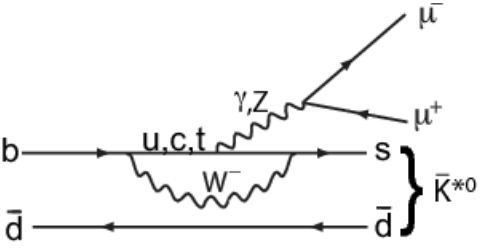
\includegraphics[scale=0.25]{content/feynman/png/BtoK1.png}
                \item []
                \item []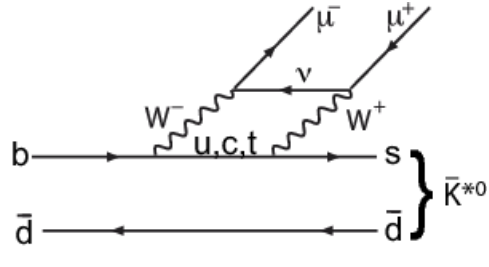
\includegraphics[scale=0.25]{content/feynman/png/BtoK2.png}
            \end{itemize}
        \end{column}
    \end{columns}
    \footnotetext[10]{arXiv:1406.6482}
\end{frame}

